\documentclass{standalone}
\usepackage{tikz}
\usepackage{ctex,siunitx,ninecolors}
\usepackage{tkz-euclide}
\usepackage{amsmath}
\usetikzlibrary{patterns, calc}
\usetikzlibrary {decorations.pathmorphing, decorations.pathreplacing, decorations.shapes,3d}
\tikzset{
pencil/.pic={
  \fill[left color =green!80!black,right color=green!80!black,middle color=white](-0.05,0.2)rectangle(0.05,1.5);
  \fill[left color =brown,right color=brown,middle color=white](-0.05,0.2)--(0,0)--(0.05,0.2);
  \fill(-0.02,0.08)--(0,0)--(0.02,0.08);
}
}
\begin{document}
\small
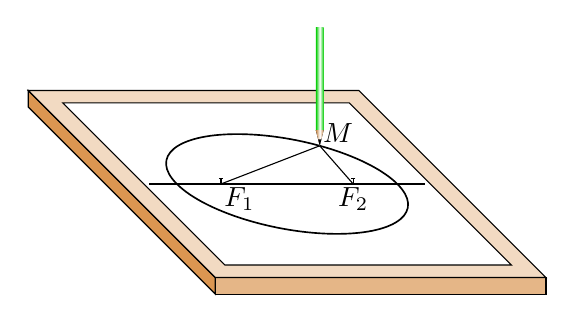
\begin{tikzpicture}[>=latex,x=(0:1cm),z=(-45:0.8cm),scale=1.4,inner sep=1pt]
  \begin{scope}[canvas is yz plane at x=-1.5]
    \draw[fill=brown7](0,-1.5)rectangle(-0.15,1.5);
  \end{scope}
  \begin{scope}[canvas is xy plane at z=1.5]
    \draw[fill=brown8](-1.5,0)rectangle(1.5,-0.15);
  \end{scope}
  \begin{scope}[canvas is xz plane at y=0]
    \draw[fill=brown9,even odd rule](-1.5,-1.5)rectangle(1.5,1.5)(-1.3,-1.3)rectangle(1.3,1.3);
    \draw[semithick](0,0)ellipse(1 and 0.8);
    \draw[thin](-1.25,0)--(1.25,0);
    \draw(0.6,0)--({cos(50)},{-0.8*sin(50)}) pic{pencil}--(-0.6,0);
    \node at ({cos(50)},{-0.8*sin(50)}) [above right]{$M$};
    \node at (-0.6,0) [below right]{$F_1$};
    \node at (0.6,0) [below]{$F_2$};
  \end{scope}
  \begin{scope}[canvas is xy plane at z=0]
    \draw(-0.6,0)--++(0,0.05)(-0.62,0.05)--(-0.58,0.05);
    \draw(0.6,0)--++(0,0.05)(0.62,0.05)--(0.58,0.05);
  \end{scope}
\end{tikzpicture}
\end{document}